\documentclass[headrule,footrule]{foils}

%%
%%%  Macros
%%%
%%% fonts-sil-charis for IPA in week 5

\newcommand{\logo}{HG2002 (2021)}
\usepackage[hidelinks]{hyperref}

\newcommand{\header}[3]{%
  \title{\vspace*{-2ex} \large 
    HG2002 Semantics and Pragmatics
% \thanks{Creative
%       Commons Attribution License: 
%       you are free to share and adapt as long as you give 
%       appropriate credit and add no additional restrictions: 
%       \protect\url{https://creativecommons.org/licenses/by/4.0/}.
%     }
    \\[2ex] \Large  \emp{#2} \\ \emp{#3}}
  \author{\blu{Francis Bond}   \\ 
    \normalsize  \textbf{Division of Linguistics and Multilingual Studies}\\
    \normalsize  \url{http://www3.ntu.edu.sg/home/fcbond/}\\
    \normalsize  \texttt{bond@ieee.org}}
  \MyLogo{\logo}
  % \MyLogo{奈良女子大学:欧米言語情報理論II}
  \date{#1
    \\  \url{https://bond-lab.github.io/Semantics-and-Pragmatics/}
\\[.5ex] \footnotesize Creative  Commons Attribution License:  you are free to share and adapt 
\\[-.25ex] \footnotesize   as long as you give    appropriate credit and add no
additional restrictions: 
\\ \small  \protect\url{https://creativecommons.org/licenses/by/4.0/}.
}
  % \renewcommand{\logo}{#2}
  % \special{! /pdfmark where
  %   {pop} {userdict /pdfmark /cleartomark load put} ifelse
  %   [ /Author (Francis Bond)
  %   /Title (#1: #2)
  %   /Subject (HG2002: Semantics and Pragmatics)
  %   /Keywords (Semantics, Pragmatics, Meaning)
  %   /DOCINFO pdfmark}
  %   }
  \hypersetup{%
    final       = true,
    colorlinks  = true,
    urlcolor    = blue,
    citecolor   = blue,
    linkcolor   = MidnightBlue,
    unicode     = true,
    pdfauthor   = {Francis Bond},
    pdfkeywords = {Semantics, Pragmatics, Meaning},
    pdftitle    = {#1: #2},
    pdfsubject  = {HG2002 Semantics and Pragmatics; License CC BY 4.0}
  }
}


\usepackage[a4paper,landscape]{geometry}
%\usepackage[dvips]{xcolor}
\usepackage[dvipsnames,x11names]{xcolor}
\usepackage{graphicx}
\newcommand{\blu}[1]{\textcolor{blue}{#1}}
\newcommand{\grn}[1]{\textcolor{green}{#1}}
\newcommand{\hide}[1]{\textcolor{white}{#1}}
\newcommand{\emp}[1]{\textcolor{red}{#1}}
\newcommand{\txx}[1]{\textbf{\textcolor{blue}{#1}}}
\newcommand{\lex}[1]{\textbf{\mtcitestyle{#1}}}


\usepackage{amsmath,latexsym}
\usepackage{pifont}
\renewcommand{\labelitemi}{\textcolor{violet}{\ding{227}}}
\renewcommand{\labelitemii}{\textcolor{purple}{\ding{226}}}

\newcommand{\subhead}[1]{\noindent\textbf{#1}\\[5mm]}

\newcommand{\Bad}{\emp{\raisebox{0.15ex}{\ensuremath{\mathbf{\otimes}}}}}
\newcommand{\bad}{*}

\newcommand{\com}[1]{\hfill \textnormal{(\emp{#1})}}%
\newcommand{\cxm}[1]{\hfill \textnormal{(\txx{#1})}}%
\newcommand{\cmm}[1]{\hfill \textnormal{(#1)}}%

\usepackage{relsize,xspace}
\newcommand{\into}{\ensuremath{\rightarrow}\xspace}
\newcommand{\ent}{\ensuremath{\Rightarrow}\xspace}
\newcommand{\nent}{\ensuremath{\not\Rightarrow}\xspace}
\newcommand{\tot}{\ensuremath{\leftrightarrow}\xspace}
\usepackage{url}
\newcommand{\lurl}[1]{\MyLogo{\url{#1}}}

\usepackage{mygb4e}
\let\eachwordone=\itshape
\newcommand{\lx}[1]{\textbf{\textit{#1}}}
\newcommand{\ix}{\ex\it}

\newcommand{\cen}[2]{\multicolumn{#1}{c}{#2}}
%\usepackage{times}
%\usepackage{nttfoilhead}
\newcommand{\myslide}[1]{\foilhead[-25mm]{\raisebox{12mm}[0mm]{\emp{#1}}}\MyLogo{\logo}}
\newcommand{\myslider}[1]{\rotatefoilhead[-25mm]{\raisebox{12mm}[0mm]{\emp{#1}}}}
%\newcommand{\myslider}[1]{\rotatefoilhead{\raisebox{-8mm}{\emp{#1}}}}

\newcommand{\section}[1]{\myslide{}{\begin{center}\Huge \emp{#1}\end{center}}}



\usepackage[lyons,j,e,k]{mtg2e}
\renewcommand{\mtcitestyle}[1]{\textcolor{teal}{\textsl{#1}}}
%\renewcommand{\mtcitestyle}[1]{\textsl{#1}}
\newcommand{\ja}[1]{\mtcitestyle{\makexeCJKactive #1\makexeCJKinactive}}
\newcommand{\chn}{\mtciteform}
\newcommand{\zsm}{\mtciteform}
%\newcommand{\cmn}[1]{make\cjkactive\mtciteform#1\makecjkinactive}
\newcommand{\iz}[1]{\textup{\texttt{\textcolor{blue}{\textbf{#1}}}}}
\newcommand{\con}[1]{\textsc{#1}}
\newcommand{\gm}{\textsc}
\newcommand{\cmp}[1]{{[\textsc{#1}]}}
\newcommand{\sr}[1]{\ensuremath{\langle}#1\ensuremath{\rangle}}
\usepackage[normalem]{ulem}
\newcommand{\ul}{\uline}
\newcommand{\ull}{\uuline}
\newcommand{\wl}{\uwave}
\newcommand{\vs}{\ensuremath{\Leftrightarrow}~}
%%% theta role
\newcommand{\tr}[1]{\textcolor{Chartreuse4}{\textsc{#1}}}
%%% theta grid
\newcommand{\grid}[1]{\ensuremath{\langle}\tr{#1}{\ensuremath{\rangle}}}

%%%
%%% Bibliography
%%%
\usepackage{natbib}
%\usepackage{url}
\usepackage{bibentry}
%\usepackage{CJKutf8}


\usepackage{fontenc}
\usepackage{polyglossia}
\setmainlanguage{english}
\setotherlanguages{tamil}
\setmainfont[Ligatures=TeX]{TeX Gyre Pagella}
\setsansfont[Ligatures=TeX]{TeX Gyre Heros}
\newfontfamily\ipafont{Charis SIL}
\newcommand\ipa[1]{\mtcitestyle{\ipafont #1}}


\usepackage{xeCJK}
\makexeCJKinactive
\newcommand{\zh}[1]{\mtcitestyle{\makexeCJKactive #1\makexeCJKinactive}}
%\newcommand{\ja}[1]{\makexeCJKactive #1\makexeCJKinactive}
\setCJKmainfont{Noto Sans CJK JP}
\setCJKsansfont{Noto Sans CJK SC}
\setCJKmonofont{Noto Sans CJK SC}

\newfontfamily\tamilfont[Script=Tamil]{Noto Sans Tamil}
\newfontfamily\tamilfontsf[Script=Tamil]{Noto Sans Tamil}
\newcommand{\tam}[1]{\texttamil{#1}}
%%% From Tim
\newcommand{\WMngram}[1][]{$n$-gram#1\xspace}
\newcommand{\infers}{$\rightarrow$\xspace}


\usepackage{rtrees,qtree}
\renewcommand{\lf}[1]{\br{#1}{}}
\usepackage{avm}
%\avmoptions{topleft,center}
\newcommand{\ft}[1]{\textsc{#1}}
\renewcommand{\val}[1]{\textit{#1}}
\newcommand{\typ}[1]{\textit{#1}}
\avmfont{\sc}
\avmvalfont{\sc}
\renewcommand{\avmtreefont}{\sc}
\avmsortfont{\it}


%%% From CSLI book
\newcommand{\mc}{\multicolumn}
\newcommand{\HD}{\textbf{H}\xspace}
\newcommand{\el}{\< \>}
\makeatother
\long\def\smalltree#1{\leavevmode{\def\\{\cr\noalign{\vskip12pt}}%
\def\mc##1##2{\multispan{##1}{\hfil##2\hfil}}%
\tabskip=1em%
\hbox{\vtop{\halign{&\hfil##\hfil\cr
#1\crcr}}}}}
\makeatletter

%\usepackage{tipa}
\usepackage{multicol}


\newcommand{\task}{\marginpar{\large ~~~\textbf{?}}}
\newcommand{\sh}[1]{\href{https://www.arthur-conan-doyle.com/index.php?title=#1}{#1}}

\usepackage{tikz}
\usepackage{tikz-qtree}
\usepackage{forest}



\begin{document}
%\begin{CJK}{UTF8}{min}
\header{Lecture 8}{Speech as Action}{}\maketitle

%\include{schedule}

\myslide{Overview}

\begin{itemize}\addtolength{\itemsep}{-1ex}
\item Revision: Context
  \begin{itemize}
  \item Knowledge as Context
  \item Information Structure
  \item Conversational Implicature
  \end{itemize}
\item Austin's Speech Act Theory
\item Categorizing Speech Acts
\item Indirect Speech Acts
%\item Sentence Types
\item Next Lecture: Chapter 9: Meaning Components
\end{itemize}

%%%
%%% this changes each year, so keep separate
%%%
\include{schedule}


\section{Revision: \\ Context and Inference}




\myslide{Context-dependence is everywhere}

\begin{itemize}\addtolength{\itemsep}{-1ex}
%\item It isn't only deictic expressions that require context
\item For example, in a bookstore
  \begin{exe}
    \ex \eng{I am looking for the new Wolfe \textnormal{[book by Wolfe]}}
  \end{exe}
\item In a snooker (pool)  game
  \begin{exe}
    \ex \eng{I have two reds left}
  \end{exe}
\item \txx{metonymy}: substituting the name of an attribute or feature for the name of the thing itself
  \begin{exe}
    \ex \eng{\ul{The ham} sandwich is at table three}
    \ex \eng{I spent all morning with \ul{the suits}}
  \end{exe}
  \item \txx{synecdoche}: substituting the name of a part for the name of a thing
  \begin{exe}
    \ex \eng{It's good to see some \ul{new faces} here}
  \end{exe}
\end{itemize}


\myslide{Knowledge as Context}
\begin{itemize}
\item Knowledge to interpret utterances can come from multiple sources
  \begin{enumerate}
  \item The physical context of the utterance
    \\ \txx{Deixis}
  \item What has already been said
    \\ \txx{Discourse}
  \item Background and common knowledge
    \\ \txx{World knowledge}
  \end{enumerate}
\item In a dialogue, we often only add new knowledge as a \txx{fragment}
  \begin{exe}
    \ex 
    \begin{xlist}
      \ex \eng{Who moved these chairs?}
      \ex \eng{Sandy (did)}
  \end{xlist}
\end{exe}
\end{itemize}

% \myslide{Discourse Topic}

% \begin{itemize}
% \item It is much easier to understand an utterance if you know what
%   they are talking about.

% \item Giving the same text different titles changes your interpretation
% \item Giving a discourse topic aids in understanding and retention
% \end{itemize}

% \myslide{Background Knowledge}

% What knowledge do we need to interpret the following?

% \begin{exe}
%   \ex 
%   \begin{xlist}
%     \ex \eng{I'm hungry
%     \ex \eng{I'll lend you some money
%   \end{xlist}
%   \ex 
%   \begin{xlist}
%     \ex \eng{Shall we get some icecream?
%     \ex \eng{I'm on a diet
%   \end{xlist}
%   \ex 
%   \begin{xlist}
%     \ex \eng{Shall we lunch next week?
%     \ex \eng{It's Ramadan
%   \end{xlist}
%  \ex 
%   \begin{xlist}
%     \ex \eng{Kim chased the dog with a stick
%     \ex \eng{Kim chased the dog with a bone
%     \ex \eng{Kim chased the dog with a broom
%     \ex \eng{Kim chased the dog with a white tail
%     \ex \eng{Kim chased the dog with a wound

%   \end{xlist}

% \end{exe}

% %\myslide{Mutual Knowledge}

% \myslide{Formalizing Knowledge for Computers}

% \begin{itemize}
% \item There is a lot of work on making knowledge available to
%   computers so that they can interpret text
%   \begin{itemize}
%   \item Formal ontologies (knowledge-based)
%     \begin{itemize}
%     \item Scripts
%     \item Wordnets
%     \item CYC
%     \end{itemize}
%   \item Example-based (compare to existing examples)
%     \\ collect many fragments of existing knowledge
%   \end{itemize}
% \end{itemize}


% \myslide{Knowledge Yielding Ontologies  
%  for Transition-based Orgs}
% \MyLogo{I do this}
% \begin{center}
%   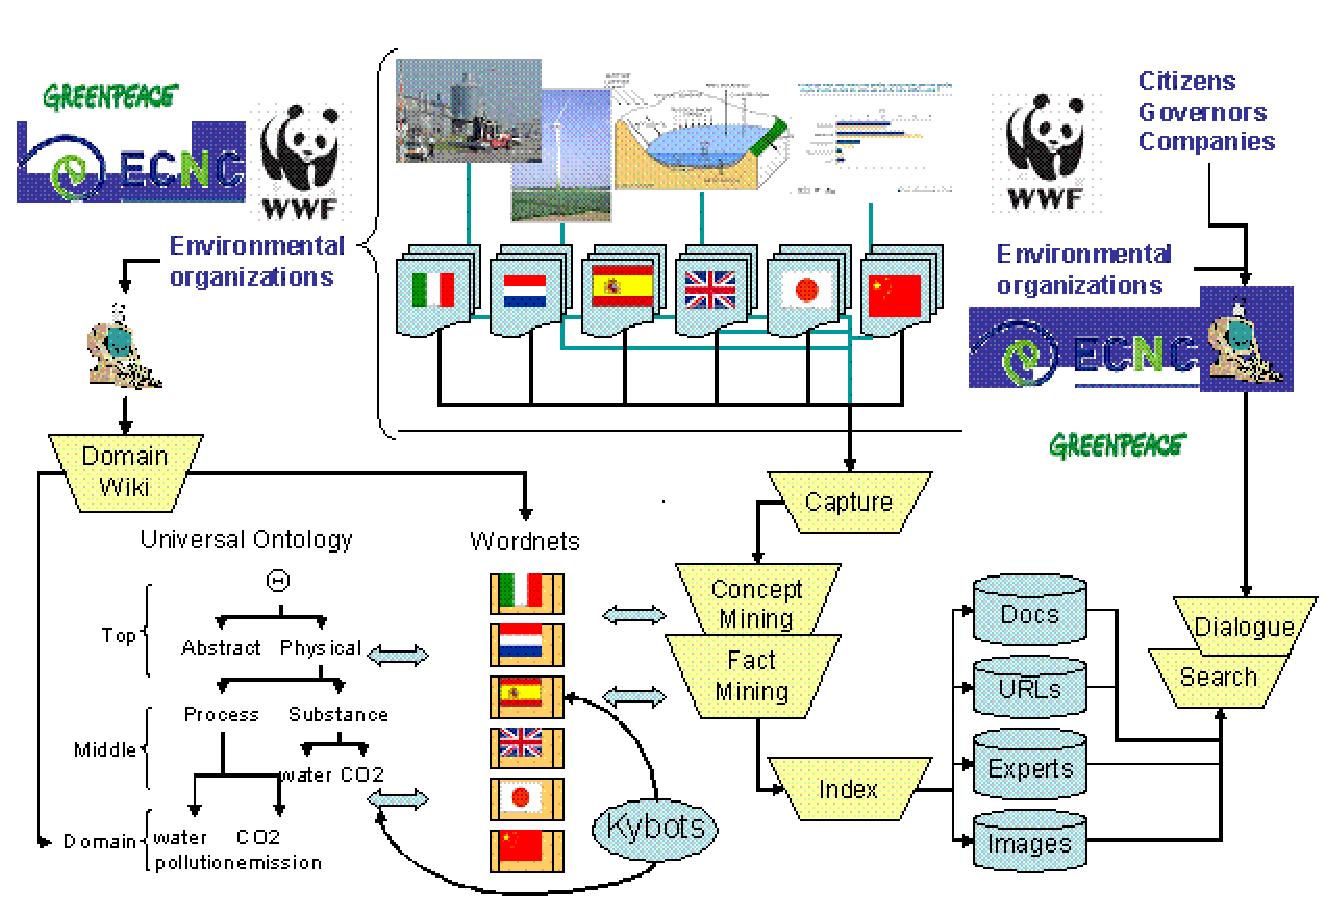
\includegraphics[width=0.8\textwidth]{pics/kyoto-project.eps}
% \end{center}

% \myslide{What can computers do?}
% \MyLogo{}
% \begin{itemize}
% \item[Q] \textit{Do birds migrate through Turkey?}
% \item[A] Yes.  \textit{The crane ($\subset$ bird) flies across Ankara ($\subset$ bird)}.
%   \begin{quote}
%     \large   fly$_1$ ($e_1$, crane$_5$($x_1$)),  across($e_2$,$e_1$,$x_2$), Ankara($x_2$).
%   \end{quote}
%   \begin{itemize}
%   \item  \textit{through} and \textit{across} are both \textit{path} roles.
%   \item \textit{fly} and \textit{migrate} are both \textit{motion} verbs.
%   \item Ankara is in Turkey
%   \end{itemize}
% \item Why do this?
%   \begin{itemize}
%   \item Local environmental knowledge often not translated into many languages
%   \item Facts may only occur in a few documents
% \end{itemize}
% \end{itemize}


\myslide{Information Structure}

\begin{itemize}
\item Many languages signal whether information is \txx{new} or \txx{given}

\item We can signal this in many ways:
  \begin{itemize}
  \item Determiners in English
  \item Intonation (focus)
  \item Topic marking
  \end{itemize}
\end{itemize}



\myslide{Cooperation in Conversation}
\begin{itemize}
\item \txx{Cooperative Principle}: people cooperate in conversation
  \begin{quote}
    ``Make your conversational contribution such as is required, at the stage at which it occurs, by the accepted purpose or direction of the talk exchange in which you are engaged.''
  \end{quote}
\item \txx{Implicature}
  \begin{quote}
    The aspect of meaning that a speaker conveys, implies, or suggests
    without directly expressing.
  \end{quote}
 \eng{Can you pass  the salt?} may implicate ``pass me the salt''
\end{itemize}

\myslide{Gricean Maxims}
\begin{small}
\begin{description}
\item [\txx{Maxim of Quantity}] ~
  \begin{itemize}
  \item Make your contribution as informative as is required
    \\ (for the current purposes of the exchange).
  \item Do not make your contribution more informative than is required.
  \end{itemize}
\item [\txx{Maxim of Quality}] ~
  \begin{itemize}
  \item Do not say what you believe to be false.
  \item Do not say that for which you lack proper evidence.
  \end{itemize}
%\newpage
\item [\txx{Maxim of Relation}] ~
  \begin{itemize}
  \item Be relevant.
  \end{itemize}
\item [\txx{Maxim of Manner}] ~
  \begin{itemize}
  \item Be perspicuous [= be easily understood]
  \item Avoid obscurity of expression.
  \item Avoid ambiguity
  \item Be brief (avoid unnecessary prolixity)
  \item Be orderly
  \end{itemize}
\end{description}
\end{small}

\myslide{Conversational Implicatures and Hedges}
\begin{itemize}
\item \txx{Generalised conversational implicatures}
\\ the inferences we make by assuming cooperation
\item \txx{Particularised conversational implicatures}
\\ local inferences for a given situation
\item \txx{Scalar implicatures (Horn Scales)}
\\ one item on  a scale implicates all weaker items (and no stronger ones)
\item \txx{Conventional implicatures}
\\ implicatures attached to lexical items
\item \txx{Hedges}: show we know we are flouting a maxim
\end{itemize}

\myslide{Horn Scales}
\newcommand{\horn}[1]{\ensuremath{\langle}\,#1\,\ensuremath{\rangle}}
\newcommand{\set}[1]{\{#1\}}
\begin{itemize}
\item Two words  ($S$ and $W$) form a Horn scale \horn{$S,W$} if: 
  \begin{enumerate}
  \item[(i)] $A(S)$ must entail $A(W)$ for some arbitrary sentence frame $A$;
  \item[(ii)] $S$ and $W$ must be equally lexicalized;
  \item[(iii)] $S$ and $W$ must be about the same semantic relations, or
    from the same semantic field. 
\end{enumerate}
\item Words on the scale implicate the negation of words on their left
  \begin{itemize}
  \item \horn{\eng{always, often, sometimes}}.
  \item \horn{\eng{\ldots, 5, 4, 3, 2, 1}}.
  \item \horn{\eng{hot, warm, lukewarm, cold}}.
  \item \horn{\eng{the},  \set{\eng{a},\eng{some}}}.
  \end{itemize}
\end{itemize}


\section{Austin's Speech Act Theory}

\myslide{Speech as Action}
\MyLogo{\citet{Austin:1962}}
\begin{itemize}
\item Language is often used to \emp{do} things: \txx{speech acts}
  \\ language has both
  \begin{itemize}
  \item \txx{interactivity}
  \item \txx{context dependence}
  \end{itemize}
\item E.g. If you greet someone or ask them a question, and they don't
  respond it is very awkward
\end{itemize}

\myslide{Sentence Types}
\MyLogo{A bit like tense and time}
\begin{itemize}
\item There are four syntactic types that correlate closely to pragmatic uses

  \begin{tabular}{lcl}
  \txx{declarative}  &$\leftrightarrow$& \txx{assertion} \\
  \txx{interrogative} &$\leftrightarrow$& \txx{question} \\
  \txx{imperative} &$\leftrightarrow$& \txx{order} \\
  \txx{optative} &$\leftrightarrow$& \txx{wish}
  \end{tabular}
\item But it turns out there is a lot of flexibility:
  \begin{exe}
    \ex \begin{xlist} 
      \ex \eng{Would you like a beer?}\hfill question
      \ex \eng{Is the pope Catholic?} \hfill assertion
    \end{xlist}
  \end{exe}
\end{itemize}

\myslide{Language as Truth}
\begin{itemize}
\item One tradition of semantics is based on these assumptions
  \begin{itemize}
  \item the basic sentence type is declarative
  \item language is mainly used to describe the world
  \item meaning can be given in terms of truth values
  \end{itemize}
\item What about these?
  \begin{exe}
    \ex \eng{Excuse me!}
    \ex \eng{Hello.}
    \ex \eng{How much can a Koala bear?}
    \ex \eng{Six pints of lager and some nachos, thanks!}
    \ex \eng{How 'bout them niners?}
  \end{exe}
\end{itemize}

\myslide{Perfomative Utterances}

\begin{exe}
  \ex \eng{I promise I won't drive home}
  \ex \eng{I bet you 5 bucks they get caught }
  \ex \eng{I declare this lecture over} 
  \ex \eng{I warn you that legal action will ensue}
  \ex \eng{I name this ship \ul{the Nautilus}}
\end{exe}

\begin{itemize}
\item Uttering these (in an appropriate context) \emp{is} acting
\\  \emp{Utterances themselves can be actions}
\item In English, we can signal this explicitly with \lex{hereby}
\end{itemize}

\myslide{Felicity Conditions}
\begin{itemize}
\item Performatives (vs Constantives) \hfill (Austin)
\\ Given the correct \txx{felicity conditions}
  \begin{description}
  \item[A1] There must exist an accepted conventional procedure that
    includes saying certain words by certain persons in certain
    circumstances,
  \item[A2] The circumstances must be appropriate for the invocation
  \item[B1] All participants must do it both correctly
  \item[B2] \ldots  and completely
  \item[C1] The intention must be to do this the act
  \item[C2] The participants must conduct themselves so subsequently.
  \end{description}
\item If the conditions don't hold, the speech act is \txx{infelicitous}
  \begin{itemize}
  \item Failing \textbf{A} or \textbf{B} is a \txx{misfire}
  \item Failing \textbf{C} is an \txx{abuse}
  \end{itemize}
  \end{itemize}

\myslide{Examples of Infelicities}
\begin{itemize} \addtolength{\itemsep}{-2ex}
\item \textbf{A1} \eng{I hereby marry you} (said by someone not authorized to do so)
\item \textbf{A2} \eng{I baptize this baby Harold} (baby’s name should Herman)
\item \textbf{A2} \eng{I pronounce John Smith dead} (uttered by a doctor who has confused John Smith
with John Smit, or if John Smith is still alive)
\item \textbf{B1}
\eng{Yes} (exchanging vows in a Christian marriage ceremony)
\item \textbf{B1}
\eng{OK} (in response to \eng{Do you swear to tell the truth, the whole truth and nothing but
the truth?} – wrong formula)
\item \textbf{B2}
\eng{I bet you \$50 the opposition loses the next election} (infelicitous without a response: \eng{OK – you’re on}; Austin calls the required response uptake)
\item \textbf{C1}
\eng{Guilty as charged} (if accused known to be innocent by a jury member)
\item \textbf{C2}
\eng{I promise to come tomorrow} (if there is no intention to keep to the promise)
\end{itemize}


\myslide{Explicit and Implicit Performatives}
\begin{itemize}
\item \txx{Explicit Performatives}
  \begin{itemize}
  \item Tend to be first person
  \item The main verb  is a performative: 
    \lex{promise, warn, sentence, bet, pronounce, \ldots}
  \item You can use \lex{hereby}
  \end{itemize}
\item \txx{Implicit Performatives}
  \begin{exe}
    \ex \eng{You are hereby charged with treason} [by me]
    \ex \eng{Students are requested to be quiet in the halls} [by NTU]
    \ex \eng{10 bucks says they'll be late} [I bet you] 
    \ex \eng{Come up and see me some time!} [I invite you]
  \end{exe}
  Can be made explicit by adding an active perfomative verb
\end{itemize}

\myslide{Elements of Speech Acts}
\begin{description}
\item \txx{Locutionary act} the act of saying something
\item \txx{\underline{Illocutionary act}} the force of the statement 
\item \txx{Perlocutionary act} the effects of the statement
\end{description}
Illocutionary force indicating devices(IFID)
\begin{itemize}
\item   word order
\item    stress
\item    intonation contour
\item    punctuation
\item    the mood of the verb
\item     performative verbs: \eng{I (Vp) you that \ldots} 
\end{itemize}

\myslide{Searle's speech act classification}
  \begin{description}
  \item \txx{Declarative} changes the world (like performatives)
  \item \txx{Representative} describes the (speaker's view of the) world 
  \item \txx{Expressives}  express how the speaker feels
  \item \txx{Directives} get someone else to do something
  \item \txx{Comissives} commit oneself to a future action
  \end{description}

% \myslide{Felicity Conditions for Promising}
% \MyLogo{Searle (1969)}

% \begin{itemize}
% \item \textbf{Preparatory 1}: $H$ would prefer $S$'s doing $A$ to his
%   not doing $A$, and $S$ believes $H$ would prefer his doing $A$ to
%   his not doing $A$.
% \item \textbf{Preparatory 2:} It is not obvious to both $S$ and $H$
%   that $S$ will do $A$ in the normal course of events.
% \item \textbf{Propositional:} In expressing that $p$, $S$ predicates a
%   future act $A$ of $S$
% \item \textbf{Sincerity:}  $S$ intends to do $A$ 
% \item \textbf{Essential:} The utterance $e$ counts as an undertaking to do $A$
% \end{itemize}

%   \begin{tabular}{llll}
%     $S$ & Speaker & $A$ & Future Action \\
%     $H$ & Hearer  & $p$ & proposition expressed \\
%         &          & $e$ & linguistic expression  
%   \end{tabular}

\myslide{Felicity Conditions for Requesting}
\MyLogo{Searle (1969), simplified}
These things must hold for an utterance to be a \txx{request}:
\begin{itemize}
\item \textbf{Preparatory 1}: $H$ is able to perform  $A$
\item \textbf{Preparatory 2}: It is not obvious that the $H$ would perform $A$  without being asked
\item \textbf{Propositional:} $S$ predicates a future act $A$ of $H$
\item \textbf{Sincerity:}  $S$ wants $H$ to do $A$ 
\item \textbf{Essential:} The utterance $e$ counts as an attempt by $S$ to get $H$ to do $A$
\end{itemize}

  \begin{tabular}{llll}
    $S$ & Speaker & $A$ & Future Action \\
    $H$ & Hearer   & $e$ & linguistic expression  \\
%        &         & $p$ & proposition expressed \\
  \end{tabular}


\section{Indirect Speech Acts}


\myslide{An example}
\MyLogo{The Big Bang Theory: An Apology Insufficiency (S4E7)}

\begin{exe}
  \ex {[Knock on the door]}
  \ex Leonard: \eng{Wanna get that?}
  \ex Sheldon: \eng{Not particularly.}
  \ex Leonard: \eng{Could you get that?}
  \ex Sheldon: \eng{I suppose I could if I were asked.}
  \trans {[Knock on the door]}
  \ex Leonard: \eng{Would you please get that?}
  \ex Sheldon: \eng{ Well of course! \\  Why do you have to make things so complicated?}
\end{exe}


\myslide{Indirect speech acts}
\MyLogo{}
\begin{itemize}\addtolength{\itemsep}{-1ex}
\item 
 \begin{tabular}[t]{lcll}
   Sentence Type & & Speech Act & Example \\ \hline
  \txx{declarative}  &$\leftrightarrow$& \txx{assertion}  (statement) & 
  \eng{I sing.}\\
  \txx{interrogative} &$\leftrightarrow$& \txx{question}  &
  \eng{Do you sing?}   \\
  \txx{imperative} &$\leftrightarrow$& \txx{order} (request, command) &
  \eng{sing!} \\
  \txx{exclamative}&$\leftrightarrow$&  \txx{exclamation} & \eng{What a voice!}  \\
  \txx{optative} &$\leftrightarrow$& \txx{wish} & \eng{If only I could sing}
  \end{tabular}
  % \begin{description}
  % \item[statement] declarative:  \eng{I sing.}
  % \item[command] imperative: \eng{sing!}  
  % \item[question] interrogative: \eng{Do you sing?}  
  % \item[exclamation] exclamative: \eng{What a voice!}  
  % \end{description}
\item Properties of Indirect Speech Acts:
  \begin{itemize}
  \item Multiplicity of meanings
  \item Logical priority of meaning
  \item Rationality
  \item Conventionality
  \item Politeness
  \item Purposefulness
  \end{itemize}
\end{itemize}  

\myslide{Literal and non-literal uses}

\begin{exe}
  \ex
  \begin{xlist}
    \ex \eng{Could you get that? }
    \ex \eng{Please pass the salt.}
  \end{xlist}
  \ex 
  \begin{xlist}
    \ex \eng{I wish you wouldn't do that.}
    \ex \eng{Please don't do that.}
  \end{xlist}
  \ex
  \begin{xlist}
    \ex \eng{You left the door open.}
    \ex \eng{Please close the door.}
  \end{xlist}
\end{exe}
\begin{itemize}
\item People have access to both the literal and non-literal meanings
\item Non literal meanings can be slower to understand
\item Some non-literal uses are very conventionalized 
  \\ \eng{Can/Could you X?} \into \eng{Please X}
\item Questioning the felicity conditions produces an indirect version
\end{itemize}

\myslide{Indirect Requests}

\begin{small}
  \begin{itemize}
\item \textbf{Preparatory 1}: $H$ is able to perform  $A$
\item \textbf{Preparatory 2}: It is not obvious that the $H$ would perform $A$  without being asked
\item \textbf{Propositional:} $S$ predicates a future act $A$ of $H$
\item \textbf{Sincerity:}  $S$ wants $H$ to do $A$ 
\item \textbf{Essential:} The utterance $e$ counts as an attempt by $S$ to get $H$ to do $A$
\end{itemize}
\end{small}
  \begin{itemize}
\item \textbf{Preparatory 1}: \eng{Can you tell me the time?}
\item \textbf{Preparatory 2}: \eng{Would you let me know the time?}
\item \textbf{Propositional:} \eng{Aren't you going to start your annotation?}
\item \textbf{Sincerity:}  \eng{I wish you would answer me}
%\item \textbf{Essential:} The utterance $e$ counts as an attempt by $S$ to get $H$ to do $A$
\end{itemize}

\myslide{Why be Indirect?}

\begin{itemize}
\item Mainly for politeness

  \begin{exe}
    \ex {[Motorist to gas station attendant]}
    \begin{xlist}
      \ex \eng{You don't happen to have any change for the phone do you?}
    \end{xlist}
    \ex {[Doctor to Nurse]}
    \begin{xlist}
      \ex \eng{I'll need a 19 gauge needle, IV tubing and some unobtanium}
    \end{xlist}
  \ex {[Teacher to student?]}
    \begin{xlist}
      \ex \eng{Would you be so kind as to give me a hand with this?}
    \end{xlist}
  \end{exe}
\item[$\Rightarrow$] Low Status \into High Status is generally more indirect than High \into Low 
\end{itemize}

\myslide{Politeness and Face-Threatening Acts}
\MyLogo{\citet{Brown:Levinson:1987}}
\begin{itemize}
\item \txx{Positive Face} desire to seem worthy and deserving of approval
\item \txx{Negative Face} desire to be autonomous, unimpeded by others
\item Threats to another’s face
  \begin{itemize}
  \item to positive: disapproval, disagreement, interruption
  \item to negative: orders, requests, suggestions
  \end{itemize}
\item Face-saving acts: 
  \begin{itemize}
  \item don't threaten another’s face: \eng{I may be wrong but, \ldots}
  \item allow for negative face: \eng{Could you please, \ldots}
  \end{itemize}
\item Is politeness trans-cultural?
\end{itemize}

%\section{Sentence Types}


\myslide{Acknowledgments and References}
\MyLogo{}
\begin{itemize}
\item Video from \textit{The Big Bang Theory} Season 4 Episode 7 ``The
  Apology Insufficiency'' %% 6:22
\end{itemize}
% \item Definitions from WordNet: \url{http://wordnet.princeton.edu/}
%  \item Some slides use material from Alexander Coupe
%  \item Strict/sloppy identity joke adapted from \textit{Literal-Minded Blog:
% Linguistic commentary from a guy who takes things too literally}.
% \\ \footnotesize\url{http://literalminded.wordpress.com/2011/03/04/you-cant-go-from-strict-to-sloppy/}
  
%  \end{itemize}
 % \item Images from
%   \begin{itemize}
%   \item the Open Clip Art Library: \url{http://openclipart.org/}
%   \item Steven Bird, Ewan Klein, and Edward Loper (2009) 
%      \textit{Natural Language Processing with Python}, O'Reilly Media
%     \\ \url{www.nltk.org/book}
% \end{itemize}
% \item Problems  partially based on exercises from Saeed (2003)
% \end{itemize}

%\myslide{Bibliography}
% Reading: Jurafsky and Martin (2008) Chapter 20
\small
\bibliographystyle{aclnat}
\bibliography{abb,mtg,nlp,ling}

%\clearpage
%\end{CJK}
\end{document}


%%% Local Variables: 
%%% coding: utf-8
%%% mode: latex
%%% TeX-PDF-mode: t
%%% TeX-engine: xetex
%%% End: 
